\documentclass{beamer}
\usepackage[utf8]{inputenc}
\usepackage[norsk]{babel}
\usepackage{graphics}
\usetheme{Warsaw}
\title[Vakumkammer] % (optional, only for long titles)
{Vakumkammer}
\subtitle{Verkt\o y for testing av temperaturegenskaper hos CubeSat i vakum}
\author[Gruppe 1, TFE4850] % (TODO)
{Harald Garvik  \and Jonas Ghini \and Eivind Kvinge \\ \and Andreas Mosand \and Erlend Sigholt \and Erlend Strandvik}
\date[2014] % (optional)
{Midsemesterpresentasjon, v\aa r 2014}
\subject{TFE4850}

\begin{document}
  \frame{\titlepage}
  \begin{frame}
    \frametitle{Utgangspunkt}
    \framesubtitle{Problemet vi skal l\o se}
    \begin{itemize}%[<+->]
    	\item Det er \o nskelig \aa\ teste studentsatelittens oppf\o rsel i vakum f\o r den sendes opp
    	\item Ved mangel av atmosf\ae re vil satelitten kun tape varme via str\aa ling. Man \o nsker ikke at den overoppheter
    	\item Bidrag til satelittens temperatur er satelittens eget str\o mforbruk, og solstr\aa ling
    	\item Per dags dato m\aa\ NUTS bestille begrenset tid med vakumkammer for \aa\ teste. De m\aa\ dessuten kunne gi garantier for avgassing, ingen eksplosjoner etc. Dette begrenser mulighetene for testing 
    \end{itemize}
  \end{frame}
  \begin{frame}
    \frametitle{Gruppas sammensetning}
    \framesubtitle{Betydning for valg av prosjekt og l\o sning}
    %\begin{columns}[t]
    	%\column{.5\textwidth}
    		\begin{block}{Sammensetning}
    		\begin{itemize}
    			\item[-] To fra Elektro
    			\item[-] To fra Data
    			\item[-] En fra EMIL
    			\item[-] En fra Bygg
    		\end{itemize}
    		\end{block}
    	\pause
    	%\column{.5\textwidth}
    		\begin{block}{Prosjekt}
    		Kompetanse til b\aa de \aa\ bygge fysisk vakumkammer, sette opp
    		n\o dvendige sensorer, i tillegg til \aa programmere mikrokontroller.
    		\newline
    		\newline
    		Perfekt gruppesammensetning for \aa\ lage et form\aa lsspesifikt vakumkammer.
    		\end{block}
    %\end{columns}
  \end{frame}
  \begin{frame}
    \frametitle{Prosjektet}
    \framesubtitle{V\aa r l\o sning}
    \begin{itemize}
    	\item Vakumkammer i passe st\o rrelse for Kubesatelitten
    	\item Temperatursensorer inne i kammeret
    	\item Tilh\o rende vakumpumpe(r)
    	\item Varmekilde inne i kammeret for \aa\ simulere solstr\aa ling
    	\item Informasjon og logging til PC via microcontroller
    \end{itemize}
  \end{frame}

  \begin{frame}
    \frametitle{Fremgang}
    \framesubtitle{Hvor er vi n\aa ?}
    \begin{block}{Kammer}
    	\begin{itemize}
    		\item[-] Vi har materialer: st\aa lvegg, aluminiumslokk og -bunn
    		\item[-] Vi har backingpumpe og turbopumpe
    		\item[-] Bestemt design p\aa\ pakninger og gjennomf\o ring til pumpe
    	\end{itemize}
    \end{block}
    \end{frame}
    
    \begin{frame}
    	\frametitle{Fremgang}
    	\framesubtitle{Hvor er vi n\aa ?}
    	\begin{block}{Hardware}
    		\begin{itemize}
    			\item[-] Designet og fått produsert et kretskort. Inneholder:
					\begin{itemize}
					\item[-] Analog front-end til fire termoelementer som skal føres inn i kammer (ADC i mikrokontroller benyttes).
					\item[-] Lokal temperatursensor for kompensering til termoelementene.
					\item[-] Trykksensor.
					\item[-] Logiske utganger til styring av pumper o.l.
					\end{itemize}
    		\end{itemize}
    	\end{block}
			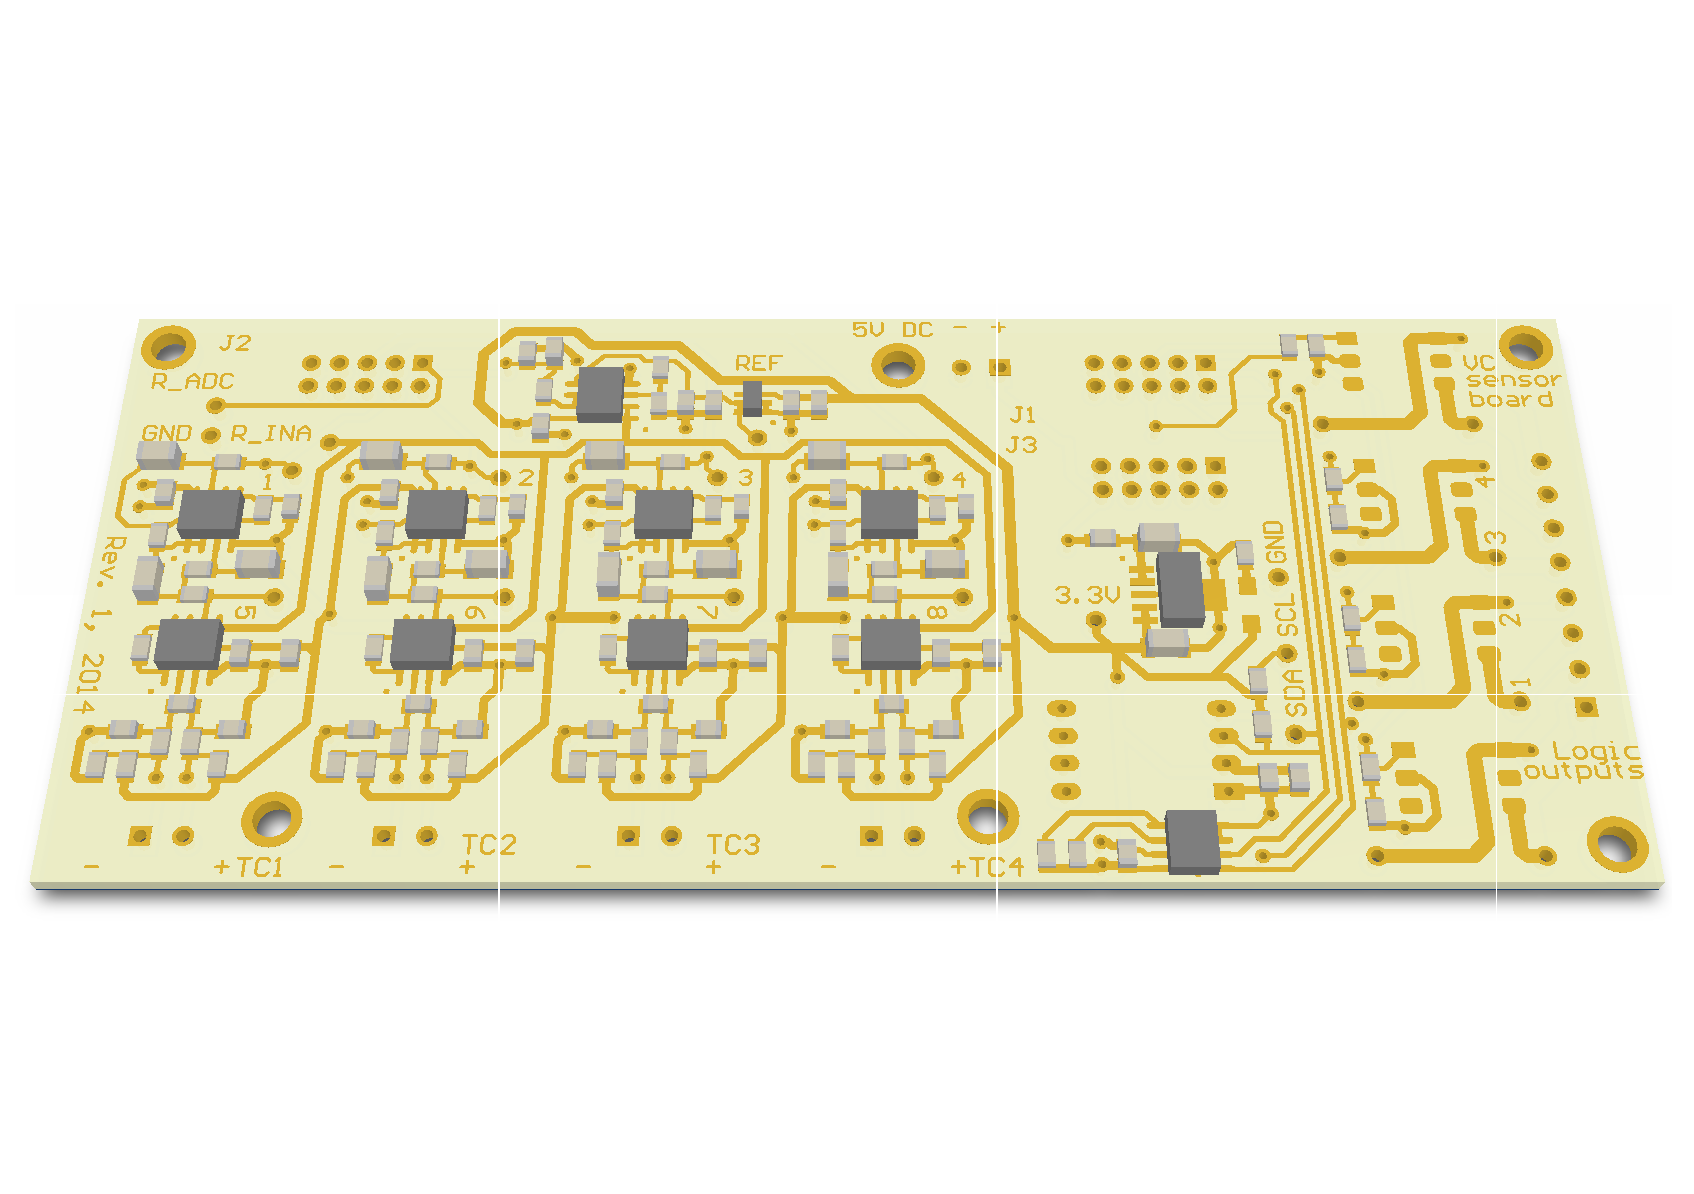
\includegraphics[width=\textwidth]{kretskort.pdf}
    \end{frame}
    
    \begin{frame}
    	\frametitle{Fremgang}
    	\framesubtitle{Hvor er vi n\aa ?}
    	\begin{block}{Software}
    		\begin{itemize}
    			\item[-] Satt opp USB-kommunikasjon via terminal, med tilh\o rende logging til fil p\aa\ PC.
    			\item[-] Konfigurert ADC (Analog Digital Converter), og satt opp st\o tte for \aa\ ta imot temperaturavlesninger fra sensorer.
    		\end{itemize}
    	\end{block}
    \end{frame}

  \begin{frame}
    \frametitle{Veien fremover}
    \framesubtitle{Hva gjenst\aa r?}
        \begin{block}{Kammer}
    	\begin{itemize}
    		\item[-] Bestemme gjennomf\o ringer til temp. m\aa ling, satellittkommuniksajon og trykkm\aa ling
    		\item[-] Maskinering: kammervegg og bunn/topp m\aa\ dreies og planeres, og topp/bunn m\aa\ få frest inn spor til O-ring
    	\end{itemize}
    \end{block}
    \end{frame}
    
    \begin{frame}
    	\frametitle{Veien fremover}
    	\framesubtitle{Hva gjenst\aa r?}
    	\begin{block}{Hardware}
    		\begin{itemize}
    			\item[-] Lodde komponenter på kretskortet, starter med en temperaturkanal.
					\item[-] Foreta målinger på temperaturkanalen, samt kalibrering.
					\item[-] Lodde resten av kortet for å teste det i sin helhet.
					\item[-] Bistå software-gruppa med kalibrering og testing av hele systemet.
    		\end{itemize}
    	\end{block}
    \end{frame}
    
    \begin{frame}
    \frametitle{Veien fremover}
    \framesubtitle{Hva gjenst\aa r?}
    \begin{block}{Software}
    	\begin{itemize}
    	\item[-] Sette opp I2C p\aa\ mikrokontroller for kommunikasjon med sensorer som skal kobles p\aa\ der
    	\item[-] Integrere sensorer med mikrokontroller n\aa r de er ferdigstilte
    	\item[-] Kalibrere sensoravlesninger
    	\item[-] Potensielt forbedre programmvare p\aa\ PC med flere features (grafisk presentasjon av logging mm.)
    	\end{itemize}
    \end{block}
  \end{frame}
  \begin{frame}
    \frametitle{Oppsummering}
    \framesubtitle{Planlagt sluttprodukt}
    \begin{itemize}
    	\item Lager fullstendig oppsett for temperaturtesting av kubesatelitten i vakuum
    	\item Totalt sett omtrent i tr\aa d med skjema
    \end{itemize}
  \end{frame}
% etc
\end{document}